\subsection{溶解度和溶解度曲线}
溶解度是考察溶液中生长晶体的最基本参数。溶解度可用在一定条件(温度、压力)下饱和溶液的浓度来表示。溶质在溶液中的浓度(溶液成分)有以下几种表示方式:
\begin{enumerate}[(1)]\itemsep -0.5ex
\item 体积摩尔浓度(mol):一升溶液中所含溶质的摩尔数。
\item 重量摩尔浓度(mol):1000g溶剂中所含溶质的摩尔数。
\item 摩尔分数($x$):溶质摩尔数对溶液总摩尔数之比。
\item 重量百分数:100g(或是1000g)溶液中所含溶质的克数。
\item 重量比:100g(或是1000g)溶剂中所含溶质的克数。
\end{enumerate}

不同的浓度表示方式适用于不同的场合。在实验室中使用(1)表示方式是很方便的,但由于和溶液体积有关,易受温度影响(某一给定的摩尔随温度升高而减小),因此在溶解度数据中,经常使用其他浓度表示法,最常用的的是重量比和摩尔分数,后者特别适于多组分混合物的成分。

在数种质组成的溶液中,某一组分的摩尔分数可表示为
\begin{equation}
x_1=\frac{m_1/M_1}{m_1/M_1+m_2/M_2+m_3/M_3+\cdots},
\end{equation}
$m$是组分的重量,$M$是其分子量。任何混合物中所有成分的摩尔分数总和等于1。

各种浓度表示法可以互相换算,对于摩尔与其他浓度表示法换算时还需知道溶液的密度。在水溶液中,当溶质含有水合物和无水合物两种形式时,其重量百分数和重量比的换算公式如下:
\begin{equation}
c_1=\frac{100c_2}{100-c_2}=\frac{100c_3}{100R-c_3}=\frac{100c_4}{100R+c_4(R-1)},
\end{equation}
其中$c_1$为100g水中所含无水物的克数,$c_2$为100g溶液中所含无水物的克数,$c_3$为100g溶液中所含水合物的克数,$c_4$为100g水中所含水合物的克数;$R=\text{水合物分子量}/\text{无水合物分子量}$。

在我们所讨论的溶液体系中,压力对溶解度影响是很小的,但温度的影响却十分显著。这种温度-浓度关系可用溶解度曲线表示。图3.3示出一些常用水溶性晶体的溶解度曲线。从图3.3中可以看出,不同物质在水中的溶解度是有明显差别的。

\begin{figure}[hpb]
 \centering
 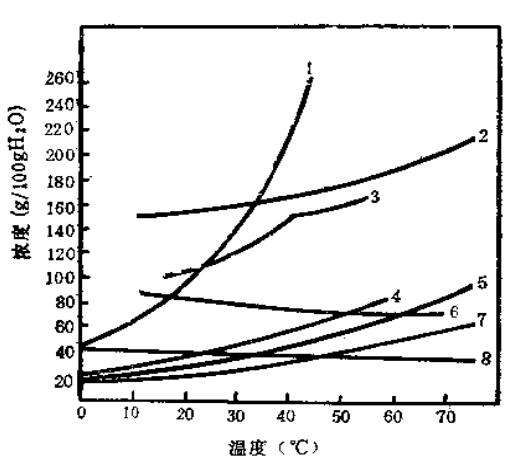
\includegraphics[width=0.8\textwidth]{fig/cp03/img3.3.jpg}
 \caption{一些水溶性晶体的溶解度曲线}
 1.酒石酸钾钠(KNT); 2.酒石酸钾(DKT); 3.酒石酸乙二胺(EDT);
 
 4.磷酸二氢铵(ADP); 5.硫酸甘氨酸(TGS); 6.碘酸锂($\rm LiIO_3$);
 
 7.磷酸二氢钾(KDP); 8.硫酸锂(LSH)。
\end{figure}

有的晶体溶解度很大,如DKT,但有的则较小,如LSH,而大多数晶体的溶解度均随温度升高而增大(溶解度温度系数为正值)。有的晶体溶解度温度系数很大(如KNT),但也有少数晶体(如LSH,Li等),溶解度的温度系数很小,而且是负值。有的晶体溶解度曲线出现拐点(如EDT),这种物质有两种不同的溶解度晶相,即EDT无水物和水合物。图3.3中所示的溶解度曲线实际上是由EDT和$\rm EDT\cdot H_2O$两条溶解度曲线组成的,这两条曲线在拐点(40.6℃)相交。该点的温度称为相平衡转变温度。

溶解度曲线是选择从溶液中生长晶体的方法和生长温度区间的重要依据。如对于溶解度及其温度系数都很大的物质,采用降温法比较理想,而对于溶解度较大,而温度系数却较小的物质则宜采用蒸发法,对于具有不同晶相的物质则需选择对所需要的那种晶相是稳定的合适的生长温度区间。

温度对溶解度的影响可用下方程式表示:
\begin{equation}
\frac{d\ln{x}}{dT}=\frac{-\Delta H}{RT^2},
\end{equation}
式中$x$为溶质的摩尔分数,$\Delta H$为固体摩尔溶解热,$T$为绝对温度,$R$为气体常量。在理想情况下,式(3.3)可化为
\begin{equation}
\log x=\frac{-\Delta H}{2.303R}\left( \frac{1}{T}-\frac{1}{T_0}\right) =\frac{-\Delta H(T_0-T)}{4.579T_0T},
\end{equation}
$T_0$为晶体的熔点。从式(3.4)中可看出:
\begin{enumerate}[(1)]\itemsep -0.5ex
\item 大多数晶体的溶解过程是吸热过程,为正,温度升高,溶解度增大。如若是放热过程,则相反。
\item 在一定温度下,高熔点晶体的溶解度小于低熔点的溶解度。
\end{enumerate}

式(3.4)也可写成
\begin{equation}
\log x = -\frac{a}{T} + b,
\end{equation}
式中$a$和$b$都是常数。

温度对溶解度的影响也可表示为
\begin{equation}
c=A+Bt+Ct^2+\cdots,
\end{equation}
式中$c$为一定量溶剂中溶质的重量,$A,B,C$是和溶液体系(溶质-溶剂)有关的常数。式(3.5)和式(3.6)是表示温度对溶解度影响的最常用的表达式。

%图3.4
\begin{figure}[hpb]
 \centering
 \subfigure[浓度(g/100g$\rm H_2O$)]{
  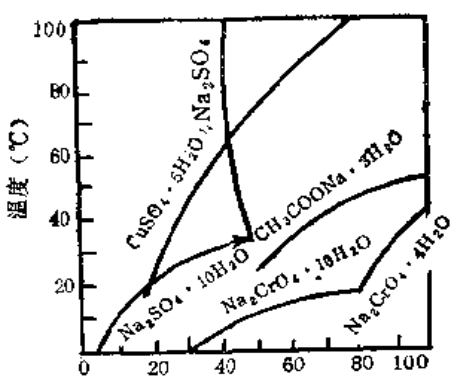
\includegraphics[width=0.6\textwidth]{fig/cp03/img3.4a.jpg}
 }
 \subfigure[无机物在水中的摩尔数(对数标尺)]{
  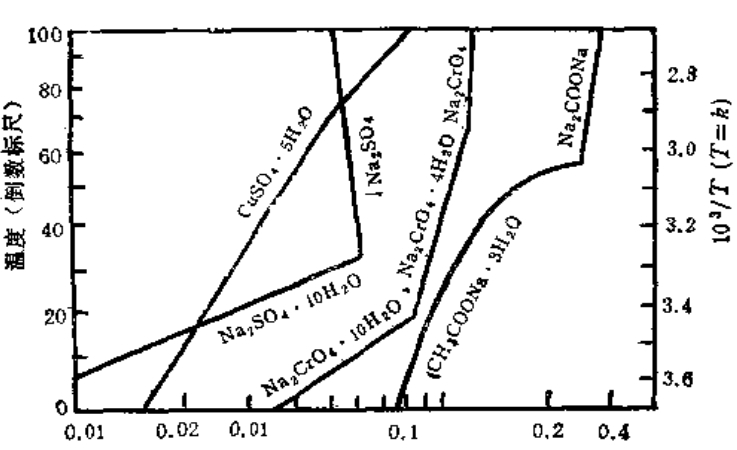
\includegraphics[width=0.6\textwidth]{fig/cp03/img3.4b.jpg}
 }
 \caption{一些盐类的溶解度曲线。}
 (a)为通常温度—浓度作图法; (b)为据式(3.5)对数坐标作图法。
\end{figure}

根据式(3.5)作图得出的溶解度曲线如图3.4(b)所示。图中的横坐标为溶质摩尔分数的对数坐标。右边纵坐标是(因为在273-373K范围内数值很小)的线性坐标。另外,也可以用专门的对数-倒数坐标图纸,将温度(℃)直接在图上标出。图3.4(b)中左边示出的纵坐标就是倒数标尺上直接标出的温度。将图3.4(a),(b)加以比较就可发现这种作图法有如下的一些优越性:
\begin{enumerate}[(1)]\itemsep -0.5ex
\item 线性好。在图3.4(a)中,在0-100℃范围内,CuSO4是平滑曲线,$\rm Na_2SO_4$和$\rm Na_2CrO_4$则分别是两条曲线在拐点(转变点)相交,而在图3.4(b)中,上述三种盐的溶解度曲线都是直线,但对一些溶解度很大的物质,或在很窄的温度区间内存在着数种水合物的物质,其溶解度仍是曲线。醋酸钠在40—50℃ 范围内直线发生弯曲,可能属于后一种情况。
\item 记录范围宽。对一些溶解度很大的盐类(如铬酸钠和醋酸钠的溶解度曲线)来说,都能像溶解度较小的盐类一样,在0-100 ℃范围内可出,这是通常的作图法无法做到的。
\item 较清楚地显示出转变点。例如通过两直线交点找$\rm Na_2SO_4$的转变点(32.4℃)要比图3.4(a)中所示延长两条曲线找转变点来得容易和准确。在图3.4(b)中,$\rm CuSO_4$的两条直线大约在67℃相交,表明硫酸铜在该处有不同的晶相转变,而在图3.4(a)中却找不出这一转变点。
\end{enumerate}

基于上述优点,利用$\log{x}-1/T$图可以用内插法和外推法求出溶解度的数值,并估计出转变温度(如果存在相平衡转变)。因此,式(3.5)在实践中很有用。